\documentclass{aa}
\usepackage{graphicx,txfonts}
\usepackage[hidelinks]{hyperref}
\journalname{Euclid Deep Field North}
\makeatletter
\renewcommand*\aa@manuscriptname{\quad\textnormal{Research report}}
\renewcommand*\aa@textidlineempty{\textit{Euclid Deep Field North}}
\AtBeginDocument{%
  \renewcommand*\aa@numarticle{}%
  \renewcommand*\aa@pageof{Page \thepage}%
}
\makeatother
\hypersetup{pdfauthor={Biswajit Jana}}
% The A&A class enables review line numbering at the end of the document.
% These are reader-facing research reports.
\renewcommand{\linenumbers}{\nolinenumbers}

\graphicspath{{../day03-cross-grism/analysis/}}
\begin{document}
\hypersetup{pdftitle={Usable H-alpha coverage in the Euclid NISP grism overlap}}
\title{Usable H$\alpha$ coverage in the Euclid NISP grism overlap}
\subtitle{Day 3. A mask and repeatability test in Euclid Deep Field North}
\author{Biswajit Jana}
\institute{Independent researcher, United Kingdom}
\date{15 November 2026}
\abstract
{The wavelength grids of the Euclid NISP blue and red grisms overlap. Usable spectral pixels and continuum coverage determine whether both can measure the same line.}
{We quantify how often the H$\alpha$ region can be fitted in both grisms and test the stability of warning-inclusive fits.}
{We join 858 Euclid DR1-Foundation sources to paired spectra in three archive partitions. We fit a fixed-centre Gaussian and a local continuum under strict and warning-inclusive masks, remove the largest red-grism core residual, and repeat selected fits at independent DESI redshifts.}
{Of 356 sources with complete nominal overlap for the adopted windows, 104 admit a strict blue fit and zero admit a strict red fit. Including pixels carrying only the low-S/N warning gives 22 dual fits and 14 with adjusted S/N $\geq5$ in both grisms. After removing one red core bin, five red fits remain above the threshold, one falls below it, and eight fail coverage. Two candidates retain a dual detection at their DESI redshift.}
{Nominal wavelength overlap substantially overstates the strict usable overlap for this sample. The warning-inclusive candidates are suitable for exposure-level follow-up.}
\keywords{methods: data analysis -- techniques: spectroscopic -- galaxies: statistics}
\maketitle
\section{Introduction}
Paired NISP spectra offer a direct comparison of a line region observed in the blue (BGS) and red (RGS) grisms. Slitless extraction can be affected by trace overlap, spectral quality masks, and residual calibration systematics \citep{copin2026,fumana2026}. The H$\alpha$ region can also contain [N\,II] from spatially distinct emission \citep{gabarra2026}. This study measures the attrition between wavelength-grid overlap and actual line fits in the Day 2 field. The target list is conditioned on the earlier pipeline H$\alpha$ selection, so the exercise tests repeatability of catalogue features.

\section{Sample and methods}
Three checksum-verified IRSA HATS partitions supply one BGS and one RGS spectrum for 858 objects in the 1576-object Day 2 parent sample \citep{aussel2026}. The fit uses a linear continuum and Gaussian width $\sigma=30$~\AA{} at $\lambda=6564.61(1+z_{\rm SPE})$~\AA. Both grids must contain the full $\pm250$~\AA{} window. A fit requires at least five usable pixels and at least 60\% usable coverage in the $\pm45$~\AA{} core, usable pixels on both sides of the centre, and at least five pixels in each 125--250~\AA{} sideband. Usable pixels have quality $>0.8$, positive variance, at least one contributing extraction and mask 0. The sensitivity fit also admits pixels with mask 2 alone.

The adjusted S/N divides the formal diagonal-variance S/N by the larger of one and the sideband residual RMS in noise units. Dual candidates require adjusted S/N $\geq5$ in each grism. For each warning-inclusive dual candidate we remove the usable red-core bin with the largest flux-density excess above the fitted continuum, then repeat the fit and coverage checks. The independent-centre comparison uses one-to-one primary DESI galaxy matches within $0.2''$ \citep{desi2025}. Wavelength-offset controls use centres at $\pm300$ and $\pm440$~\AA{} where both strict windows fit on the grids.

\begin{figure*}[t]
\centering
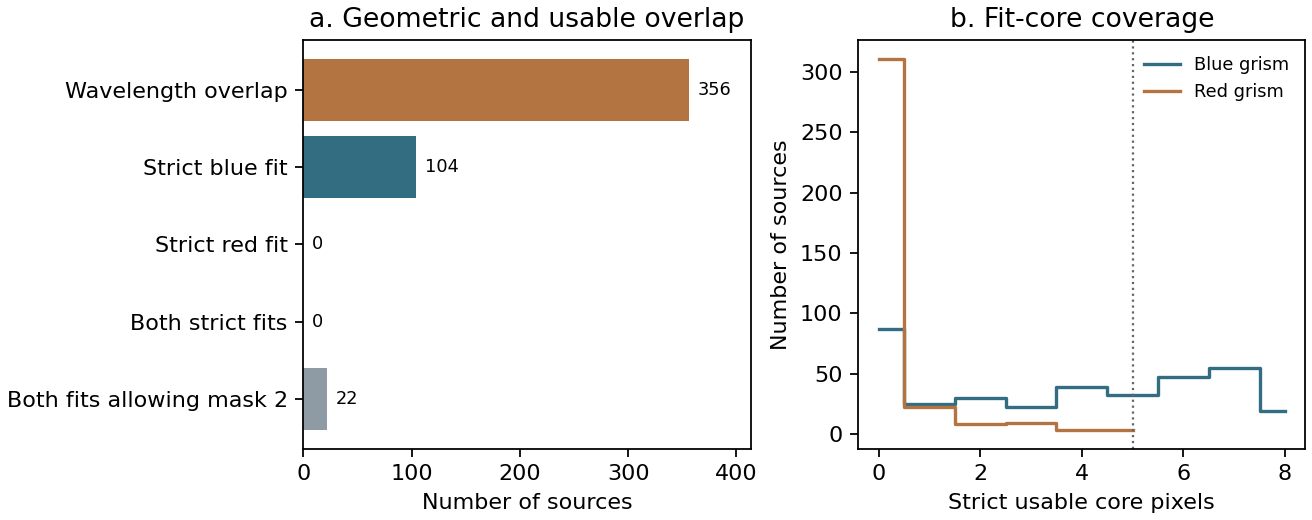
\includegraphics[width=.73\textwidth]{overlap_diagnostics.png}
\caption{Left: sources with nominal wavelength overlap and with usable fits. Right: number of strictly usable core pixels in each grism. The vertical guide marks the minimum core pixel count.}
\label{fig:coverage}
\end{figure*}

\section{Results}
The predicted centres of 407 sources lie on both grids. Requiring both full windows leaves 356 (Fig.~\ref{fig:coverage}). There are 104 strict blue fits, of which 54 reach adjusted S/N~$\geq5$. No strict red fit passes. In the red grism 311 windows have zero usable core bins, 353 have fewer than five, and 355 have fewer than five pixels in at least one sideband. These sets overlap. At the strict offset centres there is also no dual fit. The strict controls therefore cannot estimate the false-positive rate of the warning-inclusive sample.

The warning-inclusive mask gives 180 blue fits, 46 red fits, and 22 dual fits. Fourteen of the 22 reach the dual threshold. After removing the brightest red core bin, five remain above the threshold, one remains measurable below it, and eight lose fit coverage. The examples in Fig.~\ref{fig:examples} illustrate the two tests. Figure~\ref{fig:targets} shows the corresponding VIS images. The best red survivor, MER 2693214850660403334, gives adjusted red S/N 9.17 after removal. The blue and red fits for MER 2695057816657579082 reach 13.29 and 9.23 at DESI $z=0.905244$. Of three DESI galaxies among the 14 dual candidates, two pass in both grisms when re-centred on DESI. Those two lose coverage in the separate SPE-centred peak-removal test. No candidate passes both checks.

\begin{figure}[t]
\centering
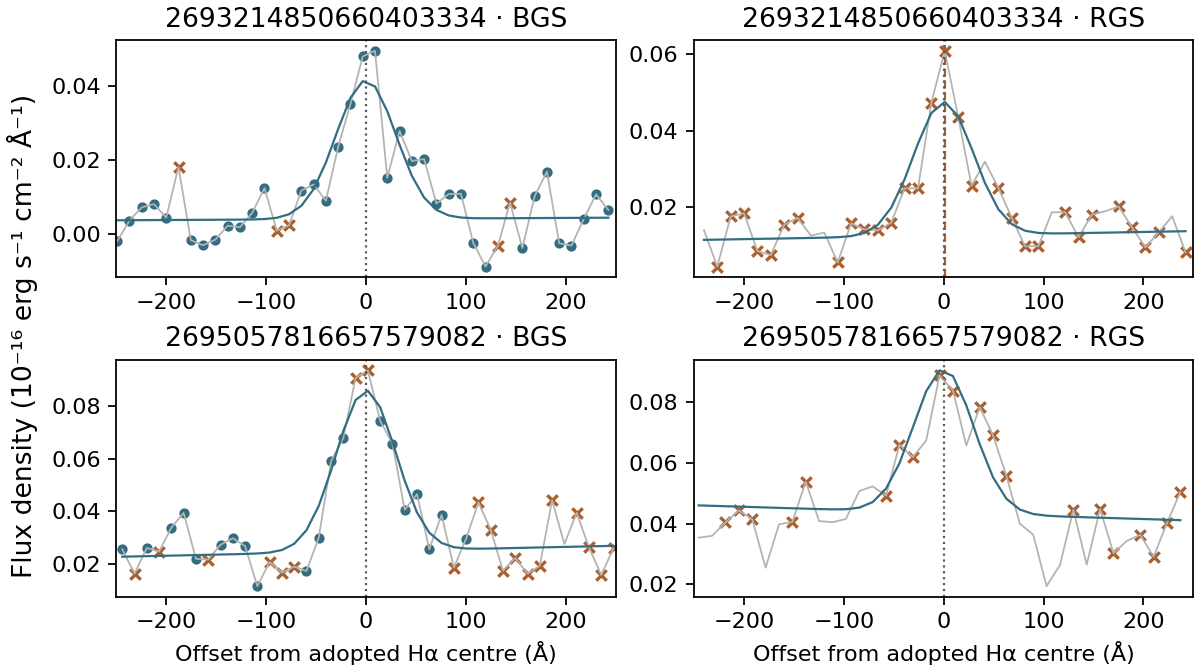
\includegraphics[width=\columnwidth]{example_spectra.png}
\caption{H$\alpha$-region fits for the strongest peak-removal survivor (top) and the strongest dual fit at a DESI redshift (bottom). Crosses mark usable pixels with mask 2. The dashed line identifies the tested red-grism bin.}
\label{fig:examples}
\end{figure}

\begin{figure}[t]
\centering
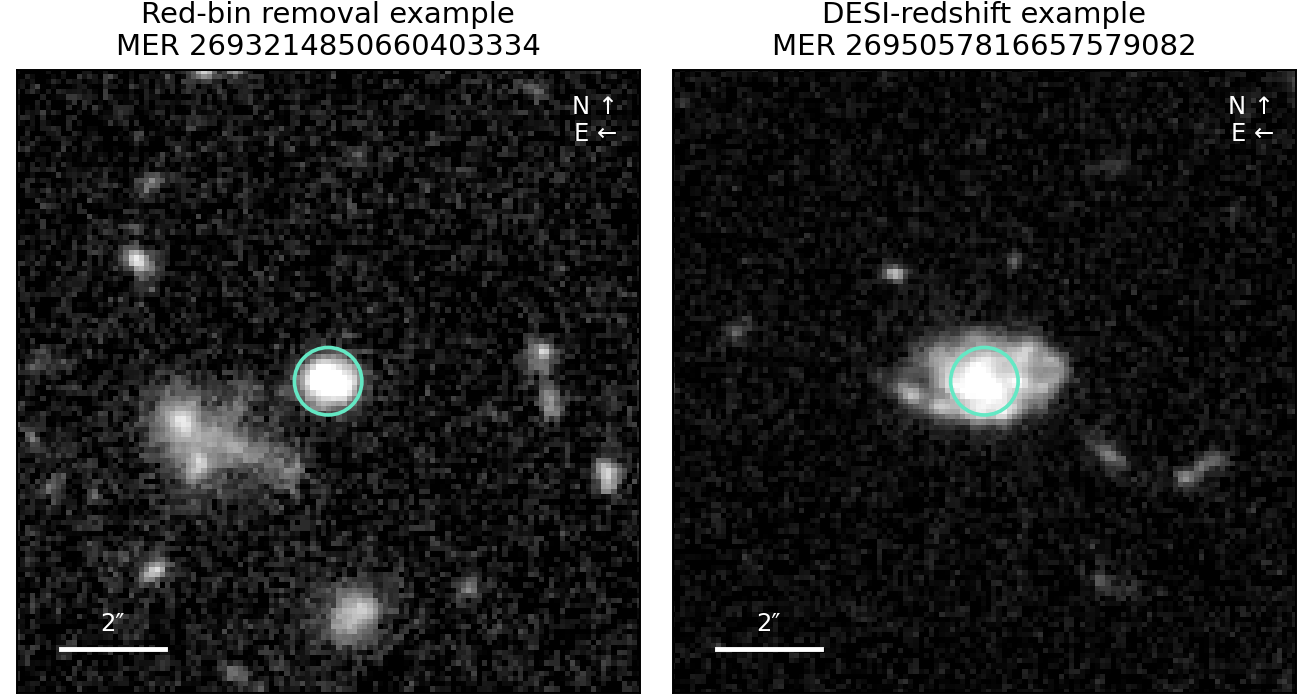
\includegraphics[width=\columnwidth]{day3_vis_targets.png}
\caption{Observed Euclid VIS thumbnails at the catalogue coordinates of the two spectral examples in Fig.~\ref{fig:examples}. Each panel spans $12''$, with north up and east left. The rings mark the MER positions.}
\label{fig:targets}
\end{figure}

\section{Discussion and conclusions}
The absence of strict red fits is a coverage result. There is no strict sample from which to estimate a blue--red flux offset. Warning-inclusive detections merit checks with individual grism orientations and two-dimensional contamination models. Selection on the pipeline line identification and the use of its redshift to position the templates limit the inference. The experiment does not establish a new object class or a new redshift for any galaxy.

\section*{Data availability}
The \href{https://github.com/Biswajit1999/daily-astro-notebooks/tree/master/euclid-dr1-foundation/day03-cross-grism}{repository} includes code, exact archive keys, checksums, fits, and the red-bin removal table. The Euclid SIR combined spectra have IRSA DOI \href{https://doi.org/10.26131/IRSA680}{10.26131/IRSA680}.
\begin{acknowledgements}
This work has made use of the Data Release (DR1) data from the Euclid mission of the European Space Agency (ESA), distributed by NASA/IPAC IRSA. DESI DR1 was accessed through NOIRLab Astro Data Lab.
\end{acknowledgements}
\bibliographystyle{aa}
\bibliography{references}
\end{document}
